\documentclass{article}
% General document formatting
\usepackage[margin=0.7in]{geometry}
\usepackage[parfill]{parskip}
\usepackage[utf8]{inputenc}
\usepackage{graphicx}
\usepackage{enumitem}

% Related to math
\usepackage{amsmath,amssymb,amsfonts,amsthm,bm, cancel}

% \newcommand{\ddx}[1][f{(x)}]{\frac{d}{dx}\left(#1\right)}
% cartesian
\newcommand{\xhat}{\hat{\textbf{x}}}
\newcommand{\yhat}{\hat{\textbf{y}}}
\newcommand{\zhat}{\hat{\textbf{z}}}
\newcommand{\rhat}{\hat{\textbf{r}}}
\newcommand{\thetahat}{\hat{\bm{\theta}}}
\newcommand{\phihat}{\hat{\bm{\phi}}}
\newcommand{\vphihat}{\hat{\bm{\varphi}}}
\newcommand{\shat}{\hat{\textbf{s}}}
\newcommand{\del}{\vec{\nabla}}

\title{Physics 408\\[0.5em]
	Build Your Own Problems\\
}
\author{Max Varverakis}

\begin{document}
\maketitle

\section*{\underline{Griffiths 1.34}}
This problem is a modification of Griffiths 1.34. The original problem asks us to verify Stokes' theorem for the vector function $\vec{v} = (xy)\xhat + (2yz)\yhat + (3zx)\zhat$ using the triangular surface made by connecting vertices $(0,0,0)$, $(0,2,0)$, and $(0,0,2)$. In the original problem, the integrals are shown to be
\begin{equation}
	\int_{S}(\del\times\vec{v})\cdot d\vec{a} = \oint_{C}\vec{v}\cdot d\vec{l} = -\frac{8}{3}.
\end{equation}

\subsection*{Adaptation}
I want to modify the surface that we use to test Stokes' theorem. In particular, I want to connect the points $(0,2,0)$ and $(0,0,2)$ by a circular arc.

\subsection*{Solution}
The figure below depicts the modified surface. Each path segment is labeled with a number.
\begin{figure}[htpb]
	\centering
	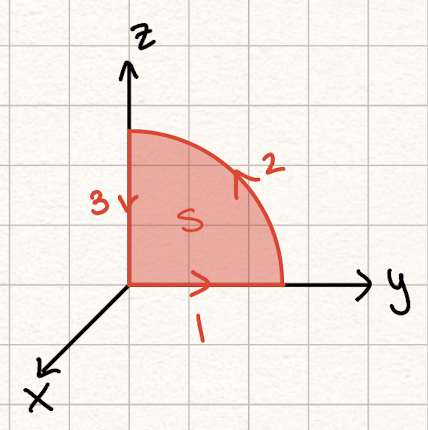
\includegraphics[width = .25\textwidth]{1.34.png}
\caption{Modified surface for Stokes' theorem.}
\end{figure}

First, let's calculate the surface integral. We have the following:
\begin{itemize}
	\item $d\vec{a} = dydz\xhat$ as by the right-hand rule convention.
	\item $\del\times\vec{v} = (-2y)\xhat + (-3z)\yhat + (-x)\zhat = (-2y)\xhat + (-3z)\yhat + 0\cdot\zhat$ since $x=0$ for this surface. Therefore, $(\del\times\vec{v})\cdot d\vec{a} = (-2y)dydz$.
	\item Note that the upper integration bound for $y$ is $\sqrt{4-z^2}$ since path 2 is an arc from a circle of radius $2$ centered at $(0,0,0)$ with corresponding equation $y^2 + z^2 = 4$.
\end{itemize}
The surface integral is then
\begin{equation}
	\int_S(\del\times\vec{v})\cdot d\vec{a} = \int_0^2dz\int_0^{\sqrt{4-z^2}}(-2y)dy = -\frac{16}{3}.
	% \int_0^1dz\int_0^{\sqrt{4-z^2}}(-2y)dy = -\int_0^1 y^2\Big|_0^{\sqrt{4-z^2}} dz
\end{equation}

Next, we calculate the integral over the boundary of the surface. Since $d\vec{l} = \xhat dx + \yhat dy + \zhat dz$, it follows that
\begin{equation}
	\vec{v}\cdot d\vec{l} = (xy)dx + (2yz)dy + (3zx)dz = 2yz dy
\end{equation}
with the simplification due to $x=0$.

Let's calculate the line integral over each path segment:
\begin{enumerate}
	\item For path $(1)$, $x=z=dx=dz=0$ where $y:0\to2$. Plugging in, this gives $\vec{v}\cdot d\vec{l} = 0$. Clearly, this path segment does not contribute to the line integral. In other words, 
	\begin{equation}
		\int\vec{v}\cdot d\vec{l} = 0.
	\end{equation}
	
	\item For path $(2)$, $x=dx=0$. We parameterize $y$ in terms of $z$ by $y = \sqrt{4-z^2}$ where $z:0\to2$. Thus, $dy = -\frac{z}{\sqrt{4-z^2}}dz$. Now, in terms of our parameterization, we can rewrite $\vec{v}\cdot d\vec{l} = 2yzdy = -2z^2dz$. Therefore, the line integral over path $(2)$ is
	\begin{equation}
		\int\vec{v}\cdot d\vec{l} = -2\int_0^2z^2dz = -\frac{16}{3}.
	\end{equation}

	\item Lastly, we have to integrate over path $(3)$. We have $x=y=dx=dy=0$ and $z:2\to0$. Thus, $\vec{v}\cdot d\vec{l} = 0$ after plugging in for $y$ and $dy$. Similar to path $(1)$, $\vec{v}\cdot d\vec{l} = 0 \implies \int\vec{v}\cdot d\vec{l} = 0$.
\end{enumerate}
To find the integral around the closed loop of $(1)\to(2)\to(3)$, we add the line integrals over each path segment to obtain
\begin{equation}
	\oint\vec{v}\cdot d\vec{l} = 0 - \frac{16}{3} + 0 = -\frac{16}{3}.
\end{equation}

Both the surface and line integrals are equal to $-\frac{16}{3}$, so Stokes' theorem is verified for this modified surface!
\clearpage

\section*{\underline{Griffiths 2.15}}
The original problem asks us to find the electric field at the three different regions of a charged thick spherical shell with inner radius $a$ and outer radius $b$. The charge density is given by $\rho = \frac{k}{r^2}$ where $k$ is a constant. The three regions are: (i) $r < a$, (ii) $a < r < b$, and (iii) $r > b$. The electric field for these cases is solved using Gauss' law and gives the corresponding electric fields:
\begin{align*}
	\vec{E}(r<a) &= 0 \\
	\vec{E}(a<r<b) &= \frac{k(r-a)}{\varepsilon_0r^2}\rhat \\
	\vec{E}(r>b) &= \frac{k(b-a)}{\varepsilon_0r^2}\rhat.
\end{align*}

\subsection*{Adaptation}
I want to instead consider a charge distribution $\rho = \frac{k}{r^2}\cosh(r)$. The three regions are the same as before.

\subsection*{Solution}
Due to the spherical symmetry, we can still leverage the power of Gauss' law to solve for the electric field using spherical Gaussian surfaces with different radii for each of the regions:
\begin{itemize}
	\item[(i)] For $r < a$, we have $Q_\textrm{enc}=0$. Since Gauss' Law states that
	\begin{equation}
		\oint\vec{E}\cdot d\vec{a} = \frac{Q_\textrm{enc}}{\varepsilon_0}\label{eq:gauss},
	\end{equation}
	it follows that
	\begin{equation}
		\frac{Q_\textrm{enc}}{\varepsilon_0} = 0 = \oint\vec{E}\cdot d\vec{a} \implies \boxed{\vec{E} = 0}.
	\end{equation}

	\item[(ii)] Now with $a < r < b$, we find the charge enclosed by our Gaussian surface with radius $r$ by integrating over the volume encompassed in the surface. Note that we integrate from $a$ to $r$ rather than from $0$ to $r$ since we already know that no charge exists within the inner radius $a$. Furthermore, in spherical coordinates, we have a differential volume element $d\tau = r^2\sin\theta drd\theta d\phi$. Thus, integrating our charge density over the volume gives
	\begin{align*}
		Q_\textrm{enc} &= \oint_V \rho d\tau\\
		&= \int_{a}^{r} \frac{k}{r^2}\cosh(r) r'^2dr' \int_{0}^{2\pi} d\phi \int_{0}^{\pi} \sin\theta d\theta \\
		&= 4\pi k\int_a^r \cosh(r) dr' \\
		&= 4\pi k \Bigl[\sinh(r) - \sinh(a)\Bigr].
	\end{align*}
	
	Applying Gauss' Law, recall that we have conveniently chosen a Gaussian surface such that at a fixed radius the electric field is both constant and perpendicular to the surface. As a result, we can pull the electric field out of the integral and evaluate the integral over the surface area of the sphere. As a result, we just get $E$ times the surface area of our Gaussian sphere. Then we can equate this surface integral to our enclosed charge and solve for the electric field, which gives
	\begin{align*}
		\int \vec{E}\cdot d\vec{a} = E\int da = E 4\pi r^2 = \frac{Q_\textrm{enc}}{\varepsilon_0} = \frac{4\pi k}{\varepsilon_0} \Bigl[\sinh(r) - \sinh(a)\Bigr].
	\end{align*}
	Simplifying, we get
	\begin{equation}
		\boxed{\vec{E} = \frac{k}{\varepsilon_0r^2}\Bigl[\sinh(r) - \sinh(a)\Bigr]\rhat},
	\end{equation}
	where we attach an $\rhat$ to the electric field since we have already determined that the electric field is radial.

	\item[(iii)] Lastly, for $r > b$, we can easily determine $Q_\textrm{enc}$ since the entire charge is enclosed by our Gaussian surface. Thus, we are now integrating over the volume of our Gaussian sphere from $r=a$ to $r=b$, which describes the charge enclosed as $4\pi k \Bigl[\sinh(b) - \sinh(a)\Bigr]$. Applying Gauss' Law, we get
	\begin{align*}
		&\int \vec{E}\cdot d\vec{a} = E\int da = E 4\pi r^2 = \frac{Q_\textrm{enc}}{\varepsilon_0} = \frac{4\pi k}{\varepsilon_0} \Bigl[\sinh(b) - \sinh(a)\Bigr] \\
		&\implies \boxed{\vec{E} = \frac{k}{\varepsilon_0r^2}\Bigl[\sinh(b) - \sinh(a)\Bigr]\rhat}.
	\end{align*}
\end{itemize}

Plotting the electric field as a function of $r$:
\begin{figure}[htpb]
	\centering
	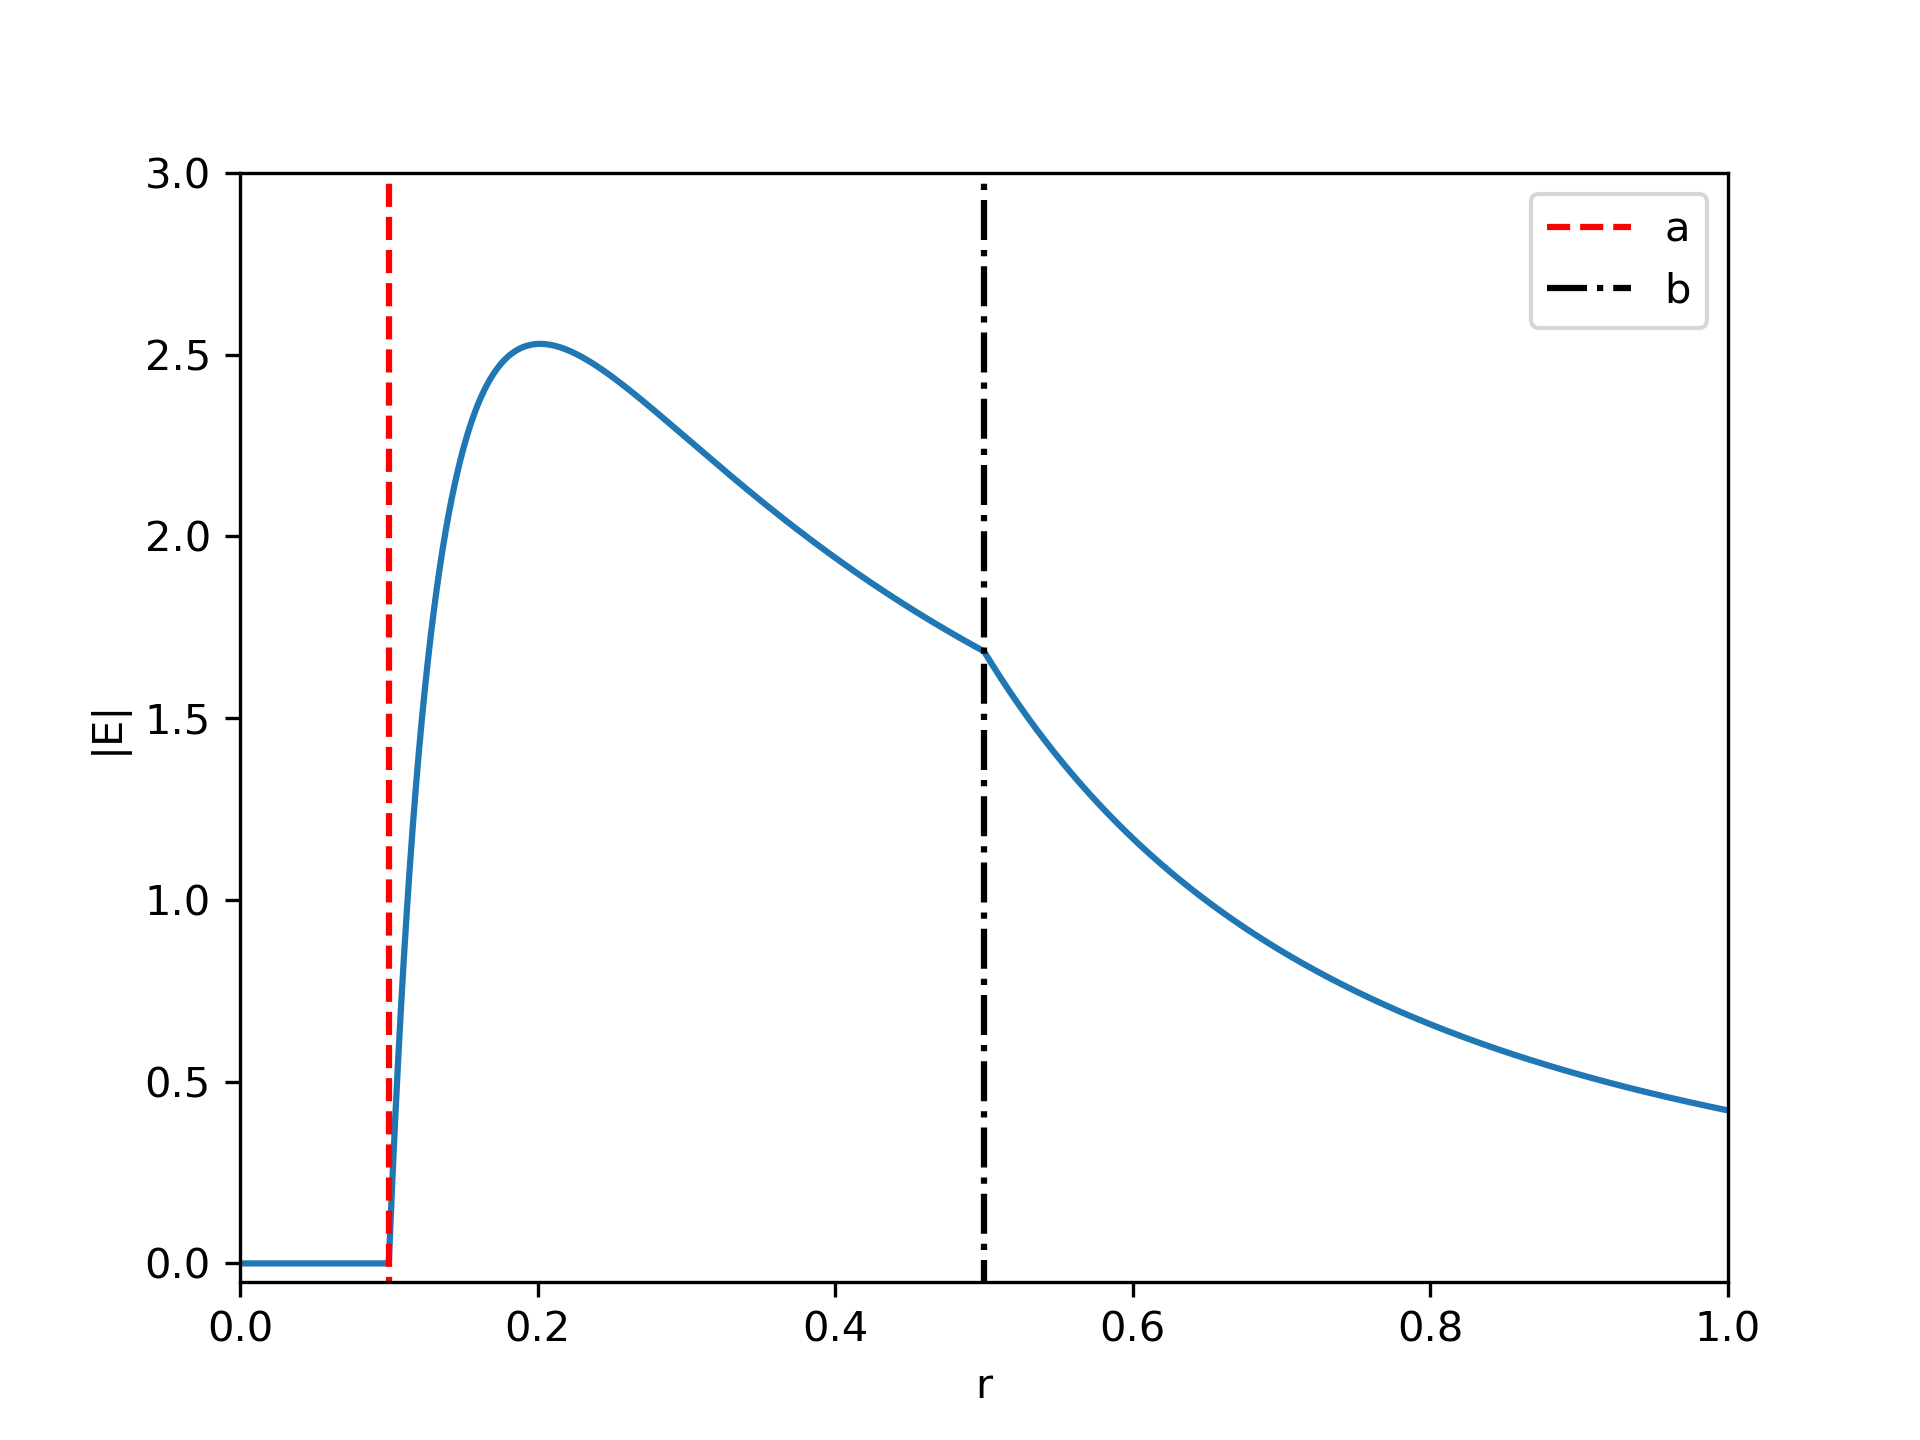
\includegraphics[width = .65\textwidth]{E_thick_shell.png}
\caption{Magnitude of electric field as a function of $r$ for a thick spherical shell with charge density $\rho = \frac{k}{r^2}\cosh(r)$.}\label{fig:thick_shell}
\end{figure}

Interestingly, there is a maximum in the electric field strength part way into the thick shell. This is due to the interplay between the decaying charge density as a function of $r$ (when $r\in(a,b)$) with the fact that $Q_\textrm{enc}$ increases as $r$ increases from $a\to b$. Furthermore, we find that the electric field is zero inside the inner radius $a$ as predicted by Gauss' Law. Outside the outer radius $b$, the electric field decays as $\frac{1}{r^2}$ as expected due to the fact that the charge enclosed is not changing after this point.

These results are similar to the original Griffiths solution in that the electric field is zero inside the inner radius $a$ and decays as $\frac{1}{r^2}$ outside the outer radius $b$. In this case, the interesting charge distribution involving $\cosh(r)$ shifted the maximum electric field strength to a point part way into the thick shell rather than at the outer boundary. However, as we can see in Figure~\ref{fig:thick_shell}, if $b$ is made close enough to $a$ (i.e., the shell is made quite thin), then the maximum electric field strength will be at the outer boundary $b$ as expected.
\clearpage

\section*{\underline{Griffiths 5.4}}
This problem has us calculate the force on a square loop (side length $a$, centered at the origin) of wire with current $I$ when placed in a magnetic field $\vec{B} = kz\xhat$, where $k$ is a constant. After some nice cancellation, we find that $\vec{F} = Ika^2$.

\subsection*{Adaptation}
I want to again find the net force on the square loop of wire, but this time with a more complicated magnetic field: $\vec{B} = \frac{kz}{\cosh(z)}\xhat$. After an in depth calculation, we will redo the problem with $\vec{B} = \frac{kz}{\sinh(z)}\xhat$ (with the hole filled at $(0,1)$). This will serve as a talking point about the symmetry of the functions and how it affects the overall solution.

\subsection*{Solution}
We first refer to the following diagram, where we have labeled four segments of the current in the square loop. We will handle each of these sections individually.

\begin{figure}[htbp]
	\centering
	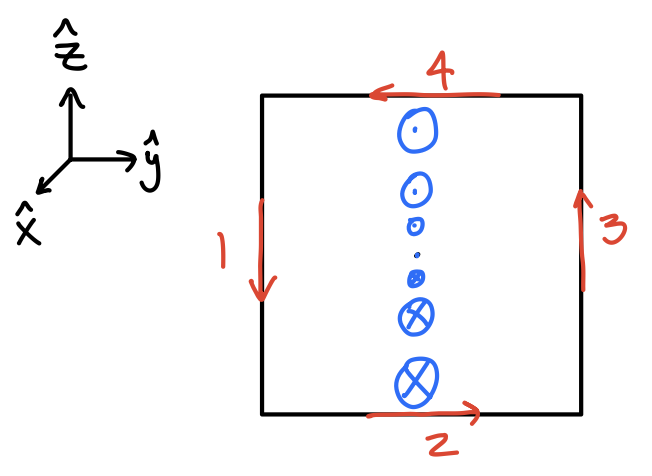
\includegraphics[width = .5\textwidth]{5.4.png}
	\caption{Schematic of square loop of wire with current $I$ in a magnetic field $\vec{B} = \frac{kz}{\cosh(z)}\xhat$. The blue serves as a visual guide for the general behavior of $\vec{B}$ inside the loop, but is not meant for analytical purposes.}\label{fig:5.4}
\end{figure}

A more detailed visualization of the magnetic field is below.
\begin{figure}[htbp]
	\centering
	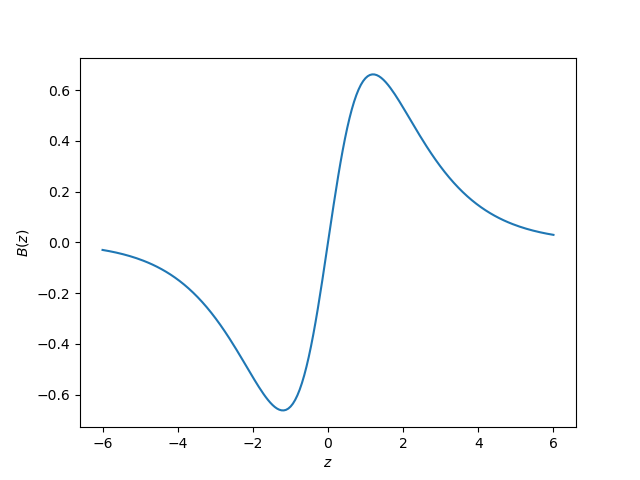
\includegraphics[width = .5\textwidth]{BFieldCosh.png}
	\caption{Magnetic field magnitude when $\vec{B} = \frac{kz}{\cosh(z)}\xhat$.}\label{fig:B_cosh}
\end{figure}

To find the total force on the loop, first recall that the force on a (constant) current-carrying wire in a magnetic field is given by
\begin{equation}
	\vec{F} = I\int d\vec{\ell}\times\vec{B}.
\end{equation}

Since the current is the same across all four labeled parts of our square loop, this gives
\begin{align}
	\vec{F}_\textrm{tot} &= I\left[ \int_1d\vec{\ell}_1\times\vec{B} + \int_2d\vec{\ell}_2\times\vec{B} + \int_3d\vec{\ell}_3\times\vec{B} + \int_4d\vec{\ell}_4\times\vec{B} \right].
\end{align}
Notice that $d\vec{\ell}_1$ is in the $-\zhat$ direction whereas $d\vec{\ell}_2$ is in the $+\zhat$ direction. For every point (defined by $z$) along wire segment 1 and 3, $\vec{B}(z)$ is the same, but their respective $d\vec{\ell}$ are in opposite directions. Therefore, the integrals over segments 1 and 3 cancel out. Similarly, $d\vec{\ell}$ for segments 2 and 4 are in opposite directions ($\yhat$ and $-\yhat$, respectively), but $\vec{B}(z)$ has opposite sign in either case (as can be seen by the blue aid drawn in Figure~\ref{fig:5.4}). Thus, due to negatives from $d\vec{\ell}$ compensating for the corresponding negative from $\vec{B}$ in the other segment, the integrals over segments 2 and 4 have the same sign. Since segment 2 is at $z=-a/2$ and segment 4 is at $z=a/2$ (and since $\vec{B}(z)$ is an odd function), the magnetic field at each of these two segments is exactly opposite by a sign. Therefore, the integrals over segments 2 and 4 are the same. Also, this means that $\vec{B}$ is constant along each of these two segments, so we can pull it outside of the integrals.

So we really only need to calculate the integral over segment 2 and multiply by 2. Along segment 2, $\vec{B}$ is in the $\xhat$ direction as can be verified by the right-hand rule.
\begin{align}
	\vec{F}_4 &= I \int_4d\vec{\ell}_2\times\vec{B} \\
	&= I \int_{\frac{-a}{2}}^{\frac{a}{2}}dy\yhat\times\vec{B}\left(z=\frac{-a}{2}\right) \\
	&= I \frac{k\left(\frac{-a}{2}\right)}{\cosh\left(\frac{-a}{2}\right)}\int_{\frac{-a}{2}}^{\frac{a}{2}}dy\yhat\times\xhat \\
	&= I \frac{k\left(\frac{-a}{2}\right)}{\cosh\left(\frac{-a}{2}\right)}\left[ \frac{a}{2} - \frac{-a}{2} \right](-\zhat) \\
	&= \boxed{I \frac{k\left(\frac{a^2}{2}\right)}{\cosh\left(\frac{a}{2}\right)}\zhat},
\end{align}
where the negative inside the argument of $\cosh$ was dropped because it is an even function. Thus, the total force on the loop is
\begin{equation}
	\boxed{\vec{F}_\textrm{tot} = 2I \frac{k\left(\frac{a^2}{2}\right)}{\cosh\left(\frac{a}{2}\right)}\zhat}.
\end{equation}

This answer agrees with our intuition on the textbook solution. The forces due to the sides of the loop cancel, and the sign change of the $\vec{B}$-field compensates for the sign change of the $d\vec{\ell}$ in the two horizontal segments, which results in a total force in the $\zhat$ direction. Although the $\vec{B}$-field in this adapted problem is more complicated, it is still odd like the original problem, so the same interaction with the segments occurs.

\clearpage
Now instead, suppose we consider $\vec{B} = \frac{kz}{\sinh(z)}\xhat$. The magnetic field magnitude is shown in Figure~\ref{fig:B_sinh}.
\begin{figure}[htbp]
	\centering
	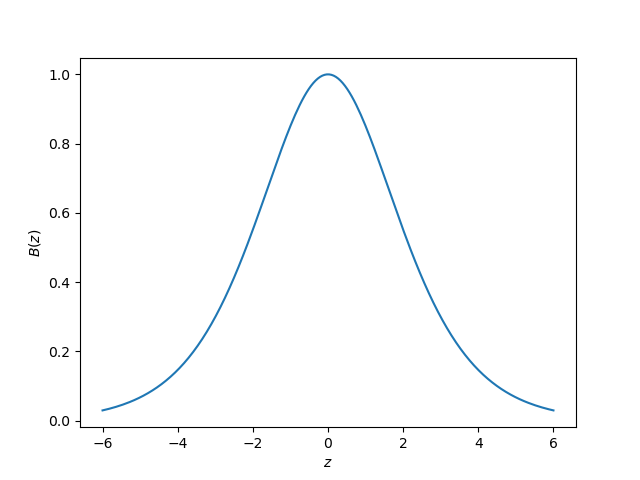
\includegraphics[width = .5\textwidth]{BFieldSinh.png}
	\caption{Magnetic field magnitude when $\vec{B} = \frac{kz}{\sinh(z)}\xhat$.}\label{fig:B_sinh}
\end{figure}

In this case, the calculation of $\vec{F}_\textrm{tot}$ is similar to the earlier calculation, however we must be cautious about negative signs. In this case, as can be seen in Figure~\ref{fig:B_sinh}, $\vec{B}(z)$ is an even function, which means that the sign of the magnetic field does not change for positive and negative $z$ values. We continue our approach to solving for $\vec{F}_\textrm{tot}$ as before, and write
\begin{align}
	\vec{F}_\textrm{tot} &= I\left[ \int_1d\vec{\ell}_1\times\vec{B} + \int_2d\vec{\ell}_2\times\vec{B} + \int_3d\vec{\ell}_3\times\vec{B} + \int_4d\vec{\ell}_4\times\vec{B} \right],
\end{align}
with the familiar labeling scheme in Figure~\ref{fig:5.4}.


Following the same argument as previously, the forces due to segments 1 and 3 (the left and right sides of the square) cancel out since the magnetic field is the same at each $z$ value along those segments, and the opposite sign of $d\vec{\ell}$ causes them to cancel at every $z$. When $\vec{B}$ was an odd function, the negative sign flipped when looking from segment 2 to segment 4. However, now the sign of $\vec{B}$ does not change when looking at segment 2 versus segment 4. This means that $\vec{B}\left(\frac{-a}{2}\right) = \vec{B}\left(\frac{a}{2}\right)$. Since $d\vec{\ell}_2 = -d\vec{\ell}_4$ as before, we have the integral over segment 2 is exactly opposite the value of the integral over segment 4. Therefore, these integrals cancel as well. We are left with zero fores on the loop, i.e. $\boxed{\vec{F}_\textrm{tot} = 0}$. 

In this particular case, things add/cancel nicely due to the magnetic field having a symmetry about the symmetries of our square loop of wire. When the magnetic fields are more complicated, however, we cannot always assume that things will cancel as they did here.

\clearpage

\section*{\underline{Griffiths 5.24}}
This original problem asks us to find the current density $\vec{J}$ that would produce the magnetic vector potential $\vec{A} = k\vphihat$, where $k$ is a constant, in cylindrical coordinates. The solution is $\vec{J} = \frac{1}{\mu_0}\frac{k}{s^2}\vphihat$, which makes sense because the current density often agrees with the direction of the magnetic vector potential.

\subsection*{Adaptation}
The adaptation of this problem involves finding the current density $\vec{J}$ that would produce the magnetic vector potential $\vec{A} = \frac{k}{s}\zhat$.

\subsection*{Solution}
First, notice that the magnetic field is related to $\vec{A}$ by a cross product:
\begin{equation}
	\vec{B} = \del\times\vec{A}.
\end{equation}
Recall that the cross product in cylindrical coordinates is
\begin{equation}
	\del\times\vec{A} = \left( \frac{1}{s}\frac{\partial A_z}{\partial \varphi} - \frac{\partial A_\varphi}{\partial z} \right)\shat + \left( \frac{\partial A_s}{\partial z} - \frac{\partial A_z}{\partial s} \right)\vphihat + \frac{1}{s}\left( \frac{\partial}{\partial s}(s A_\varphi) - \frac{\partial A_s}{\partial \phi}  \right)\zhat.
\end{equation}

Observe that the only non-zero component of $\vec{A}$ is $A_z$ which depends only on $s$. Therefore, the cross product becomes
\begin{align}
	\vec{B} = \del\times\vec{A} &= -\frac{\partial A_z}{\partial s}\vphihat = -\frac{\partial}{\partial s}\left(\frac{k}{s}\right)\vphihat = \frac{k}{s^2}\vphihat.
\end{align}

Similarly, the current density is related to the magnetic field by a cross product:
\begin{equation}
	\vec{J} = \frac{1}{\mu_0}\del\times\vec{B}.
\end{equation}

Then we can find the current density by taking the curl of our previous answer. Once again, only one term of this cross product is nonzero since there is only one component of $\vec{B}$ (namely, $\vec{B}_\varphi$), and it depends only on $s$. This yields
\begin{align}
	\vec{J} = \frac{1}{\mu_0}\del\times\vec{B} = \frac{1}{\mu_0}\del\times\left(  \frac{k}{s^2}\vphihat\right) = \frac{1}{\mu_0}\frac{\partial}{\partial s}\left( \cancel{s}\frac{k}{s^{\cancel{2}}} \right)\zhat = \boxed{-\frac{k}{\mu_0}\frac{1}{s^2}\zhat}.
\end{align}

As in the original problem, this solution makes sense intuitively because of the agreement of the direction of $\vec{J}$ and $\vec{A}$.

\clearpage

\section*{\underline{Griffiths 4.10}}
The original problem asks to find the bound charges and the electric field inside and outside a sphere of radius $R$ with polarization $\vec{P}(r) = kr\rhat$ where ${r}$ is the distance from the center of the circle. The bound surface and volume charges are equal and opposite in total, so the external electric field is zero. The internal electric field is $\vec{E} = \frac{-k}{\varepsilon_0}r\rhat$.

\subsection*{Adaptation}
I want to find the same quantities but with a polarization $\vec{P}({r}) = k{r}^2$.

\subsection*{Solution}
First, we will find the bound charges. We can use the familiar formulas to find the bound surface and volume charges:
\begin{align}
	\sigma_b &= \vec{P}\cdot\hat{\textbf{n}} = kR^2\rhat\cdot \rhat = \boxed{kR^2}, \\
	\rho_b &= -\del\cdot\vec{P} = -\frac{1}{r^2}\frac{\partial}{\partial r}\left( r^2 kr^2 \right) = \boxed{-4kr},
\end{align}
where $r$ has been replaced by $R$ for $\sigma_b$ (bound surface charges) since we are on the surface of the sphere.

Next, we can find the electric field inside and outside the sphere by using Gauss's Law (Eqn.~\ref{eq:gauss}). Note that our Gaussian surface is a sphere of radius $r$ such that the electric field is constant along the surface of the sphere (really, it's the electric flux, but the symmetry of the sphere ensures this based off of the geometry of our charge distributions).

For $r<R$, we have
\begin{align}
	\oint\vec{E}\cdot d\vec{a} &= E \cdot 4\pi r^2 \\
	&= \frac{1}{\varepsilon_0} Q_{\textrm{enc}} \nonumber\\
	&= \frac{1}{\varepsilon_0} \int_V \rho_b d\tau \nonumber\\
	&= \frac{1}{\varepsilon_0} \int_0^r \int_0^\pi \int_0^{2\pi} (-4kr') {r'}^2 \sin\theta d\phi d\theta dr' \nonumber\\
	&= \frac{-4\pi k}{\varepsilon_0}r^4 \nonumber
\end{align}
where the first equality comes from the fact that we chose a Gaussian sphere centered about our charged sphere's center. This is the same reasoning as in the solution of the adaptation of Griffith's 2.15. We already know the direction of the electric field must be radial due to the symmetry of the problem. Therefore,
\begin{equation}
	\boxed{\vec{E}(r<R) = \frac{-4\pi k}{\varepsilon_0}r^4\rhat}
\end{equation}

For the case where $r>R$, we have a much simpler setup. As can be shown using Divergence Theorem (Griffiths Problem 4.14) the charge due to the bound surface and volume charges cancels out. Thus, once our Gaussian surface encloses both the entire volume of the sphere and therefore the surface of the sphere, the total charge enclosed is zero. By Gauss's Law, this implies that
\begin{equation}
	\boxed{\vec{E}(r>R) = 0}.
\end{equation}

This solution makes sense, since we wouldn't expect to observe an electric field outside an object that was originally neutral (the bound charges are just shuffled around, but the total charge is still zero). This result does not depend on the specific mathematics of the polarization!

\end{document}